%%%%%
% ch5 %
%%%%%

\chapter{Forced and natural convection}
\section{Conduction and convection}
	\begin{wrapfigure}[10]{l}{4cm}
	\vspace{-5mm}
	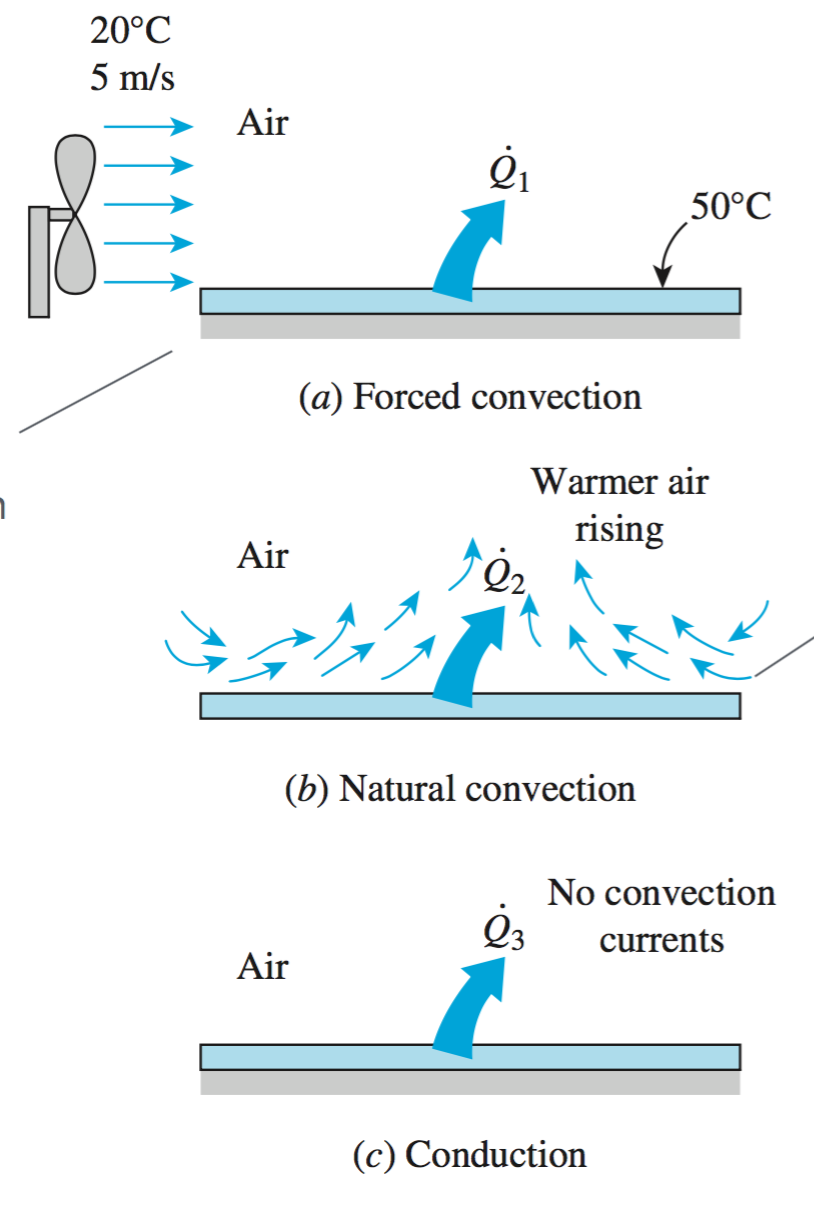
\includegraphics[scale=0.25]{ch5/1}
	\end{wrapfigure}	
	Heat transfer through a solid is always conduction, the molecules position are relatively fixed. Heat transfer in a liquid or gas is convection if there is a \textbf{bulk} fluid motion and is conduction when there isn't. Conduction in a fluid is the limiting case of convection where the fluid is \textbf{quiescient}\footnote{Au repos}.  \\
	Convection is complicated due to the fact that it involves fluid motion as well as conduction. Fluid motion \textbf{enhances}\footnote{Améliore} fluid motion, it brings the cooler and warmer part of fluid into contact, increasing the rate of heat transfer. \\
	Natural convection is caused by a density gradient. 

\section{Macroscopic energy balance}
	\begin{wrapfigure}[6]{r}{5cm}
	\vspace{-5mm}
	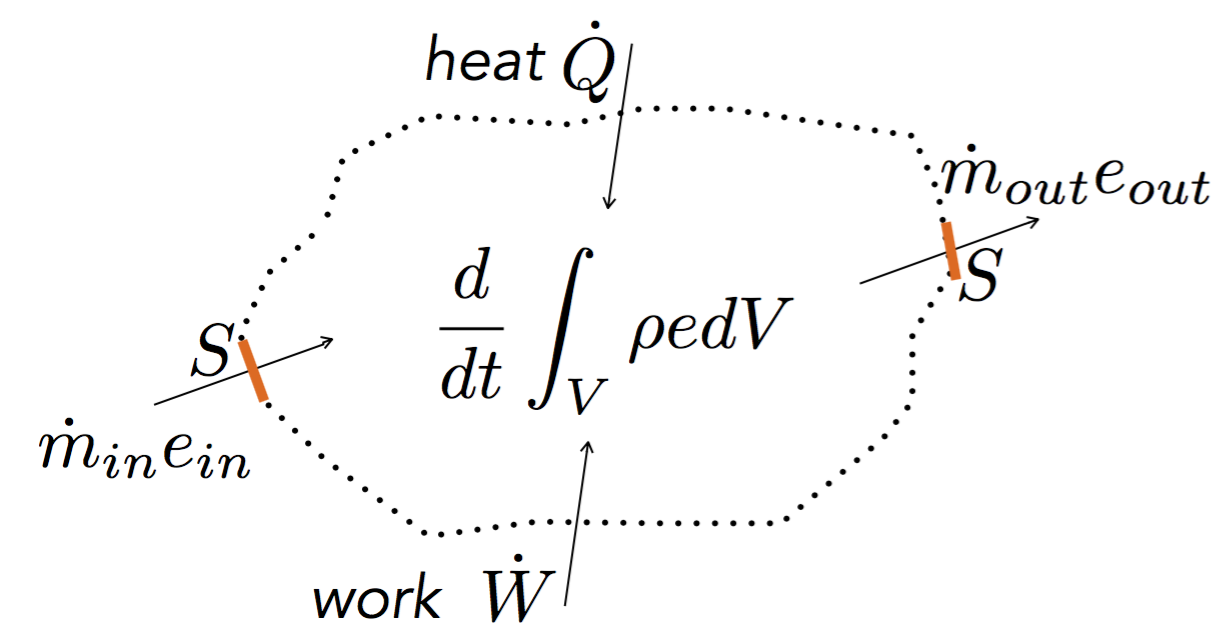
\includegraphics[scale=0.25]{ch5/2}
	\end{wrapfigure}	
	Let's consider a control volume and let's apply an energy balance, using $e = u + \frac{v^2}{2} + gz$ where the first term is the internal energy, the second the kinetic energy and the last the potential energy 
	\begin{equation}
		\frac{d}{dt}\int _V \rho e \, dV = (\rho v e S)_{in} - (\rho v e S)_{out} + \dot{W} + \dot{Q}
	\end{equation}
	Where the work can be decomposed in a \textbf{boundary} and a \textbf{useful} work and the heat is given by
	\begin{equation}
		\dot{W} = \dot{W}_f + \dot{W}_p = pvS + \dot{m}w_p = \dot{m}\left( \frac{p}{\rho}+w_p \right) \qquad and \qquad \dot{Q} = \dot{m} q
	\end{equation}		 
	The transient form is given by 
	\begin{equation}
		\frac{d}{dt}\int _V \rho e \, dV = - \Delta (\frac{1}{2}\rho v^3S) - g \Delta (\rho v z S) - \Delta (pvS) - \Delta (\dot{m}u) + \dot{m}w_p + \dot{m}q
	\end{equation}
	The steady form 
	\begin{equation}
		0 = \Delta \left( \frac{1}{2}v^2 + gz + u + \frac{p}{\rho} \right) - q - w_p 
		\label{eq:5.4}
	\end{equation}
	
	\subsection{Relation with the generalized Bernouilli equation}
		Let's take the steady form of the energy balance for a finite transformation \autoref{eq:5.4} and let's convert it for an infinitesimal transformation 
		\begin{equation}
			0 = - \left( \frac{1}{2}dv^2 + g dz + d\left(\frac{p}{\rho}\right) \right) + (\delta q - du) + dw_p
			\label{eq:5.5}
		\end{equation}
		Let's remind (see \emph{Chimie-Physique}) that the \textbf{Gibbs equation} (corresponding to elemental working change) and the \textbf{second principle} of thermdynamics are given by the expressions
		\begin{equation}
			du = Tds - pdV \qquad and \qquad Tds - \delta q= dh_f \geq 0
		\end{equation}
		Combining the two equations around $Tds$
		\begin{equation}
			\delta q - du = -dh_f + pdV
		\end{equation}
		and replacing in \autoref{eq:5.5}, we obtain the \textbf{generalized Bernouilli equation}
		\begin{equation}
			\frac{1}{2}dv^2 + g dz + \frac{dp}{\rho} = w_p - dh_f \qquad
			 \underset{\rho = cst}{\longrightarrow} \qquad 
			 \frac{1}{2}\Delta v^2 + g \Delta z + \frac{\Delta p}{\rho} = w_p - h_f 
		\end{equation}
		
	\subsection{Simplification in case of heat exchange}
		When we analize heat exchange processses, we assume that we can also consider the variation of enthalpy. We can so rewrite the expression and make appear the heat flux in function of the difference of enthalpy in the streams. So we have 
		\begin{equation}
			u + \frac{p}{\rho} = u + pv = h \qquad and \qquad \underbrace{\Delta h = \int _{T_0}^T c_p \, dT}_{Gas} \qquad \underbrace{\Delta h = c\Delta T}_{Liquid}
		\end{equation}
		We assume that thermal power is much higher than the power for pumps and compressors and that the enthalpy change is much higher than the kinetic and potential energy variation. Applying all that to equation \autoref{eq:5.4}, we have
		\begin{equation}
			\dot{Q} = \dot{m}\Delta h = \Delta \dot{H}
		\end{equation}
		
\section{The heat transfer coefficient}
	\subsection{The Nusselt number}
	\label{subsec:5.3.1}
	The rate of convection $\dot{Q}$ is proportional to the temperature difference. 
	\begin{equation}
		\dot{Q} = h S(T_p - T_f)
	\end{equation}		
	\begin{wrapfigure}[3]{l}{4cm}
	\vspace{-15mm}
	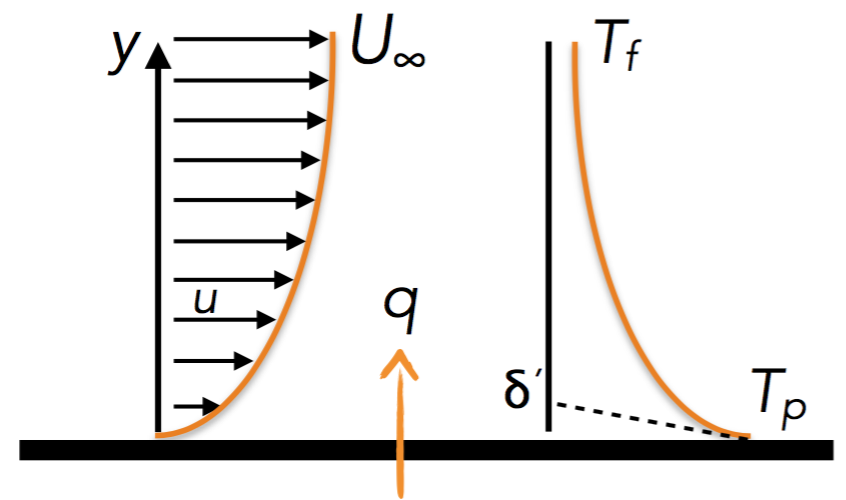
\includegraphics[scale=0.25]{ch5/3}
	\end{wrapfigure}	
	$h$ here is not the enthalpy but the \textbf{heat transfer coefficient}. Let’s give a sens. Imagine that you have a fluid flow and it is approaching a solid. The heat transfer from solid surface to the fluid layer is by pure conduction, since the fluid layer obeys the no-slip conditions. Now if you have $T_p$ miner than $T_f$ we have that type of schéma. The heat is then convected. The heat flux to the first layer is given by (where $\delta '$ is the layer thickness)
	\begin{equation}
		\dot{q}_p = -k_f \frac{\partial T}{\partial y}|_p = k_f\frac{(T_p-T_f)}{\delta '}
	\end{equation}
	Combining that with the \textbf{Newton law}, we find an expression for $h$
	\begin{equation}
		\dot{q}_p = h(T_p-T_f) \qquad \Rightarrow \qquad h = \frac{k_f}{\delta '}
	\end{equation}
 	We can non-dimentionalize that with the \textbf{Nusselt number} that gives the heat transfer enhancement thanks to convection ($Nu = 1$ represents pure conduction)
 	\begin{equation}
 		Nu = \frac{hL}{k_f}
 	\end{equation}
	
	\subsection{Comparaison with the Biot number}
		If we look to the two definition 
		\begin{equation}
			Nu = \frac{hL}{k_f} \qquad and \qquad Bi = \frac{hL}{k_s}
		\end{equation}
		They seem to be the same. Be careful because it's not the case ! Indeed the \textbf{Nusselt number} can be written as 
		\begin{equation}
			Nu = \frac{\frac{\partial (T_p - T)}{\partial y}|_p}{\frac{T_p-T_f}{L}} = \frac{\mbox{Temperature gradient at the surface}}{\mbox{Reference external temperature gradient}}
		\end{equation}
		
		\begin{wrapfigure}[4]{r}{2cm}
		\vspace{-5 mm}
		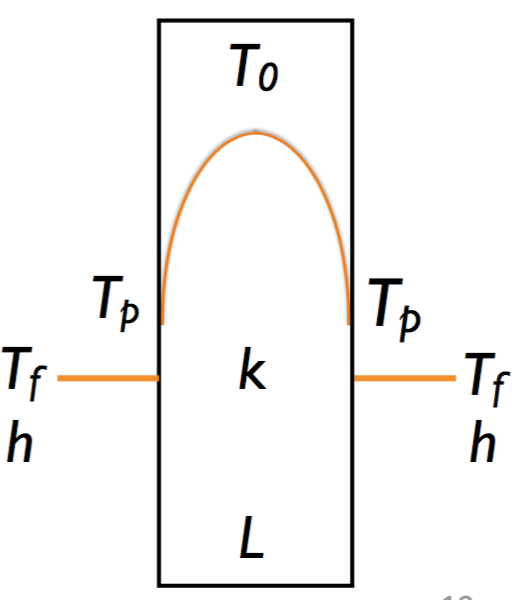
\includegraphics[scale=0.25]{ch5/4}
		\end{wrapfigure}			
		The \textbf{Nusselt number} so caracterizes the \textbf{fluid} while the \textbf{Biot number} caracterizes the \textbf{solid}
		\begin{equation}
			Bi = \frac{\frac{(T_0 - T_p)}{L}|_p}{\frac{T_p-T_f}{L}} = \frac{\mbox{Internal temperature gradient}}{\mbox{Reference external temperature gradient}}
		\end{equation}
	
	\subsection{Forced convection in pipes and channels}
	\label{subsec:5.3.3}
		We know that the heat flux is transversal to the flow (analogy with the momentum flux). Graetz proposed an analyse and here is the result
		\begin{equation}
			Nu = \frac{hD_h}{k_f}
		\end{equation}		
		Where $D_h$ is the hydraulic diameter and $k_f$ the fluid conductivity. The value for the case of a constant wall temperature or a constant heat flux are given in slide 11 chapter 5. \\
	Let's precise that for turbulent regime the Nusselt number is given by 
	\begin{equation}
	Nu = 0.023 Re^{\frac{4}{5}}Pr^n
\end{equation}		
	where $Pr$ is the \textbf{Prandtl number} (yes it's correctly written) and $n=0.4$ or $n=0.3$ respectively for a heated or cooled fluid. We remind that the Reynolds number $Re = \frac{vD}{\nu}$ compares the momentum convection to the momentum diffusion. The Prandtl number 
	\begin{equation}
			Pr = \frac{c_p \mu}{k} = \frac{c_p \mu \rho}{k\rho} = \frac{\nu}{\alpha}
	\end{equation}
	compares the momentum diffusion to the energy diffusion (wheter momentum diffuse better or not than energy). \\
	That definition of Nusselt number is limited to the range 
	\begin{equation}
		Re > 10^4 \qquad and \qquad 0.7 < Pr < 600
	\end{equation}
	\textbf{Bonus :} $RePr = \frac{vD}{\alpha}$ is the \textbf{Peclet number}

	\subsection{Laminar convection for the flow around a submerged object}
		The professor said for slide 13 that all the formula are in the formulaire and that we just have to know that there is a specific Nussel number for each case (sphere, cylinder, flat plate).
		
\section{Local form of the energy equation}
	\begin{wrapfigure}[6]{l}{3cm}
	\vspace{-5 mm}
	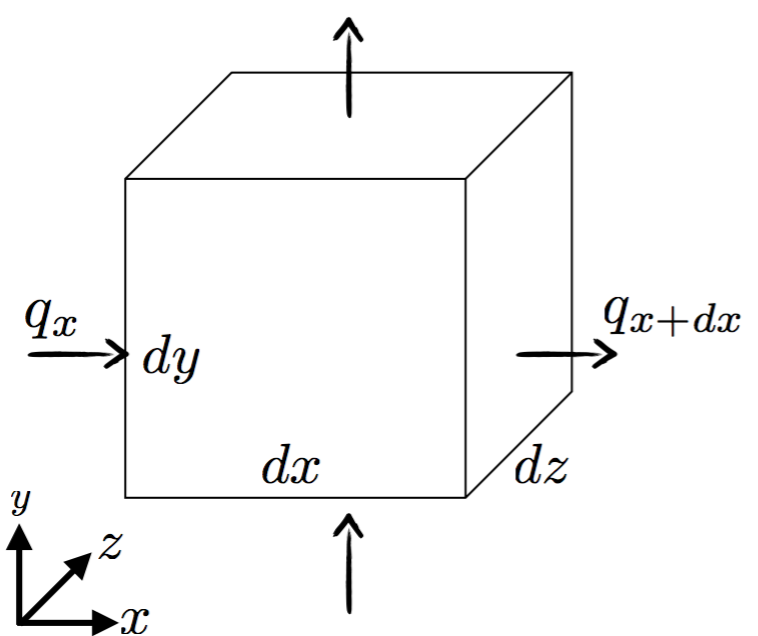
\includegraphics[scale=0.25]{ch5/5}
	\end{wrapfigure}			
	We are going to do a simple balance where the flux in and out are associated to mass flow rates and conduction. 
	\begin{equation}
		\mbox{internal energy variation} = \mbox{Heat in}-\mbox{Heat out}+\mbox{Heat source}
	\end{equation}
	The internal energy variation is given by
	\begin{equation}
		\frac{\partial (\rho cT\, dx\, dy\, dz)}{\partial t} = (\rho\, dx\, dy\, dz)\, c\frac{\partial T}{\partial t}
	\end{equation}
	the difference Heat in - Heat out due to mass tranfer by 
	\begin{equation}
		- \rho c_p (u\frac{\partial T}{\partial x} +v\frac{\partial T}{\partial y} + w\frac{\partial T}{\partial z})\, dx\, dy\, dz
	\end{equation}
	by conduction
	\begin{equation}
		- \left( \frac{\partial q_x}{\partial x} + \frac{\partial q_y}{\partial y} + \frac{\partial q_z}{\partial z} \right) dx\, dy \, dz
	\end{equation}
	and the source term 
	\begin{equation}
		\dot{Q}_v \, dx \, dy \, dz
	\end{equation}
	We put all this together and get the equation and using the \textbf{Fourrier law} for $q$
	\begin{equation}
	 \rho c\frac{DT}{Dt} + \nabla (-k\nabla T) = \dot{Q}_v \qquad or \qquad \frac{DT}{Dt} + \nabla (\alpha \nabla T) = \frac{\dot{Q}_v}{\rho c}
	 \label{eq:5.27}
	\end{equation}
	
\section{Heat transfer in pipe flows}
	\begin{wrapfigure}[6]{r}{5.2cm}
	\vspace{-5mm}
	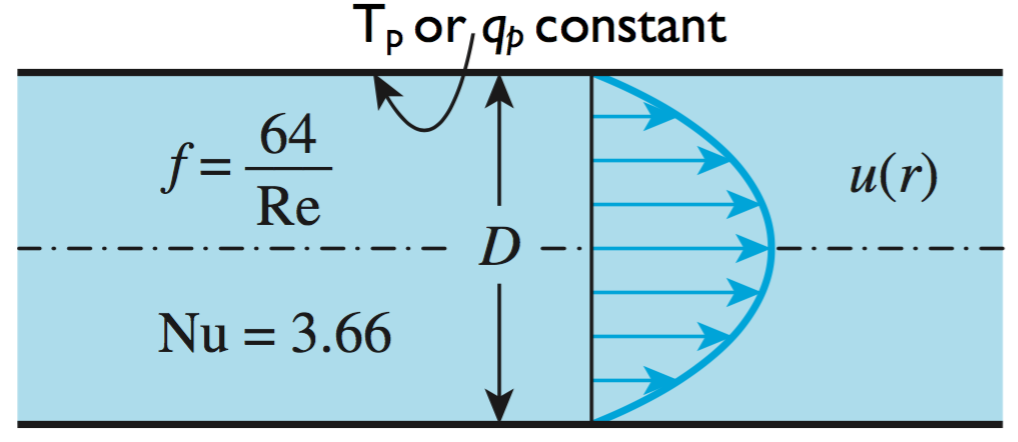
\includegraphics[scale=0.3]{ch5/6}
	\end{wrapfigure}			
	We consider a circular pipe of radius R, with constant temperature walls or constant heat flux at the walls. The flow inside is fully-developped, so the velocity is function of the radius and the friction is known. The system is steady and the flow laminar. 
	\subsection{Analysis of Graetz}
		The velocity profile is described by Poiseuille like 
		\begin{equation}
			\frac{u}{U_{max}} = 1 - \left( \frac{r}{R} \right)^2
		\end{equation}
		Using the energy equation \autoref{eq:5.27}, we can express it in polar coordinates 
		\begin{equation}
			u \frac{\partial T}{\partial x} = \alpha \left[ \frac{1}{r}\frac{\partial }{\partial r} \left( r\frac{\partial T}{\partial r}\right) + \cancel{\frac{\partial ^2 T}{\partial x^2}} \right]
			\label{eq:5.29}
		\end{equation}
		where we can neglect the last term because the diffusion in mainly in the radial direction. The boundary conditions due to the symetry and the imposed flux are 
		\begin{equation}
			r = 0 \Rightarrow \frac{\partial T}{\partial r} = 0 \qquad and \qquad
			r = R \Rightarrow \frac{\partial T}{\partial r} = -\frac{q}{k}
		\end{equation}
		Before solving we have to do a consideration. The heat flux $q$ and $h$ are constant everywhere on the wall. So the velocity only change in the vertical direction. We express that, noting the mean temperature variation $<T>$, like 
		\begin{equation}
			\dot{m}c \frac{d <T>}{dx} = qS \Rightarrow \frac{d <T>}{dx} = \frac{qS}{\dot{m}c} = C_0
		\end{equation}
		Giving the final equation for \autoref{eq:5.29}
		\begin{equation}
			\alpha \frac{1}{r}\frac{\partial }{\partial r} \left( r\frac{\partial T}{\partial r}\right) = u(r) C_0
		\end{equation}
		If we solve that we get the temperature profile ($T_c$ for temperature at centreline)
		\begin{equation}
			T-T_c = \frac{C_0 U_{max}R^2}{4\alpha} \left[ \left( \frac{r}{R} \right)^2 - \frac{1}{4}\left( \frac{r}{R} \right)^4 \right]
		\end{equation}
	
	\subsection{Nusselt number for constant temperature and constant heat flux}
		See slide 20 for the formula. Just to know that the Nusselt numbers are exact values and not an approximations !  We can find the temperature of the wall by considering that. With the heat transfer coefficient we can do what ? We are able to apply the Newton’s law ! \\
		The Nusselt number changes for other geometries and other friction factors. 
		
\section{The thermal boundary layer}
\subsection{Definition}
	\begin{wrapfigure}[6]{l}{4cm}
	\vspace{-5 mm}
	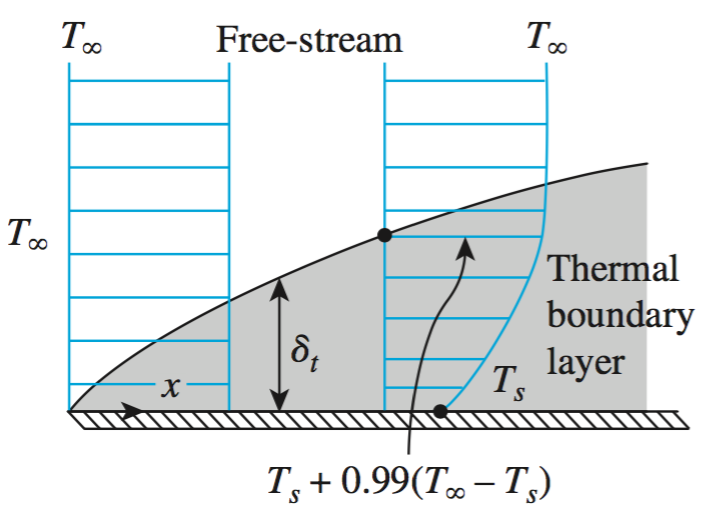
\includegraphics[scale=0.3]{ch5/7}
	\end{wrapfigure}			
	How to estimate the boundary layer thickness in a turbulent flow ? What we can see here is that if we have a high Reynolds number ($Re \gg 1$), we will develop a velocity boundary layer and a high temperature difference will develop a thermal boundary layer. Similarly to the non-sleep conditions, the fluid will be in a temperature on the surface, giving a temperature profile ranged from $T_s to T_\infty$. \\
In this thermal boundary layer temperature varies in the normal direction to the plate. The boundary layer thickness $\delta _T$ is the distance at wich the difference $T-T_s = 0.99 (T_\infty -T_s)$ and increases in the flow direction. \\
Convection strongly depends on the developpement of the velocity boundary layer relative to the thermal one. 

\subsection{The Peclet number}
	We previously defined the \textbf{Peclet number} as 
	\begin{equation}
		Pe_t = \frac{J_{E_c}}{J_{E_d}} = \frac{vL}{\alpha} = RePr
	\end{equation}
	For high-velocity flows over a flat plate, the Peclet number is much higher than 1. It means that : 
	\begin{itemize}
		\item[•] Far from the wall : Convection $\gg$ Diffusion ($Re \gg$)
		\item[•] At the wall : Convection $\ll$ Diffusion ($Re \ll$)
		\item[•] At the boundary layer height : Convection = Diffusion ($Re = 1$)
	\end{itemize}
	
\subsection{Governing equations}
	For an incompressible fluid in 2 dimensions we will use : 
	\begin{itemize}
		\item[•] Continuity equation
		\item[•] Navier-Stokes along x
		\item[•] Navier-Stokes along y
		\item[•] Equation de la chaleur
		\item[•] Boundary conditions 
			\begin{equation}
				\left\{
				\begin{aligned}
				y&= 0 \Rightarrow u = v = 0 \Rightarrow T = T_0 \\
				y &\rightarrow \infty \Rightarrow u = U, v=0 \Rightarrow T = T_\infty \qquad p = p
				\end{aligned}
				\right.	
			\end{equation}
	\end{itemize}
	
\subsection{Scaling of the different terms}
	\begin{itemize}
		\item[•] Heat flux 
			\begin{equation}
				q = -k \left( \frac{d T}{d y} \right)_{y = 0} \approx -k \frac{\Delta T}{\delta _T} 
			\end{equation}
		\item[•] Nusselt number 
			\begin{equation}
				Nu = \frac{hL}{k} = \frac{L}{\delta _T}
			\end{equation}
		\item[•] Heat transfer coefficient 
	\end{itemize}
	
\subsection{Momentum vs thermal boundary layer length}
	\subsubsection{Re >> 1}
		In this case, we have the 2 boundary layer, momentum and thermal. We already know that the thickness of momentum boundary layer decreases relatively to the Reynolds number using
		 \begin{equation}
		 	\delta \approx LRe^{-\frac{1}{2}}
		 \end{equation}
		 We have 2 limiting cases (see definition of Prandtl number in subsection \ref{subsec:5.3.3}): 
		 \begin{itemize}
		 	\item[•] If $Pr \ll 1$, $\delta _T \gg \delta$ so heat diffuses very quickly compared to momentum (liquid metals)
		 	\item[•] If $Pr \gg 1$, $\delta _T \ll \delta$ so heat diffuses very slowly compared to momentum (oil)
		 \end{itemize}
		 \begin{center}
		 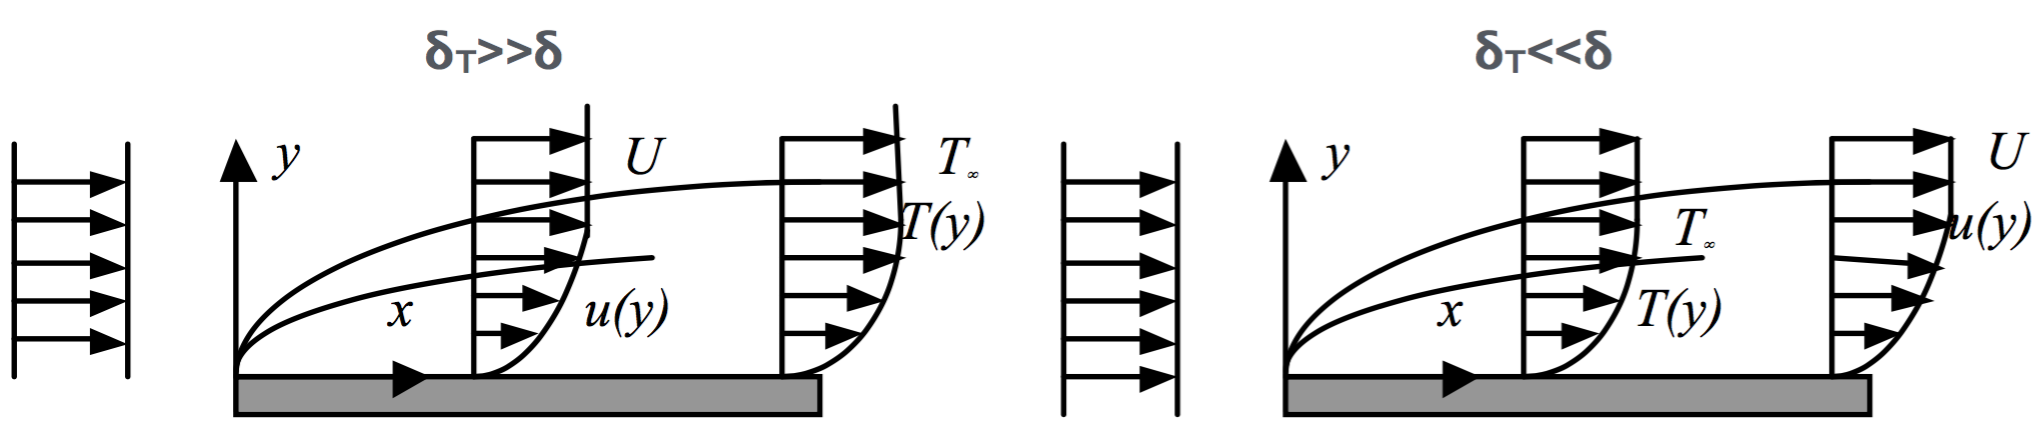
\includegraphics[scale=0.3]{ch5/8}
		 \end{center}
		 
	\subsubsection{Re >> 1 and Pr << 1}
		Let's study that case where the two boundary layer exist. We will assume that $\delta _T \gg \delta$ and verify a posteriori. The heat transfer takes place outside the momentum boundary layer so $u=U$ (fluid upcoming speed) and the velocity $v$ is obtained by \textbf{continuity equation}
		\begin{equation}
			\frac{\D u}{\D x} + \frac{\D v}{\D y} = 0 \qquad \Rightarrow \qquad v \approx U\frac{\delta _T}{L}
		\end{equation}
		The convective heat transfer terms are of the same order of magnitude 
		\begin{equation}
			u\frac{\D T}{\D x} \approx v\frac{\D T}{\D y} \approx \frac{U\Delta T}{L}
		\end{equation}
		Only the transversal diffusion term is relevant ($\delta \ll L$)
		\begin{equation}
			\alpha \frac{\D ^2 T}{\D x^2} \ll \alpha \frac{\D ^2 T}{\D y^2} \approx \frac{\alpha \Delta T}{\delta _T ^2}
		\end{equation}
		We know that at the boundary layer border convection = conduction. It allows us to calculate $\delta _T^2$ equalizing the 2 previous equations
		\begin{equation}
			\delta _T^2 = \frac{\alpha L}{U} \Rightarrow Nu = \frac{L}{\delta _T} = Pe ^{\frac{1}{2}} = Re^{\frac{1}{2}} Pr^{\frac{1}{2}} \qquad \Rightarrow  \delta _T = LRe^{-\frac{1}{2}}Pr^{-\frac{1}{2}} = \delta Pr^{-\frac{1}{2}}
		\end{equation}
		
	\subsubsection{Re >> 1 and Pr >> 1}
		Let's study that case where the 2 boundary layers exist. We will assume that $\delta _T \ll \delta$ and verify a posteriori. The heat transfer takes place \textbf{inside} the boundary layer so we assume a linear velocity profile for $u \Rightarrow u = U\frac{\delta _T}{\delta}$ in the boundary layer and the velocity $v$ is obtained by \textbf{continuity equation}
		\begin{equation}
			\frac{\D u}{\D x} + \frac{\D v}{\D y} = 0 \qquad \Rightarrow \qquad v \approx U\frac{\delta _T}{L}
		\end{equation}
		The convective heat transfer terms are of the same order of magnitude 
		\begin{equation}
			u\frac{\D T}{\D x} \approx v\frac{\D T}{\D y} \approx \frac{U\Delta T \delta _T}{\delta L}
		\end{equation}
		Only the transversal diffusion term is relevant ($\delta \ll L$)
		\begin{equation}
			\alpha \frac{\D ^2 T}{\D x^2} \ll \alpha \frac{\D ^2 T}{\D y^2} \approx \frac{\alpha \Delta T}{\delta _T ^2}
		\end{equation}
		We know that at the boundary layer border convection = conduction. It allows us to calculate $\delta _T^2$ equalizing the 2 previous equations
		\begin{equation}
			\frac{\delta _T^3}{\delta} = \frac{\delta _T^3}{LRe^{-\frac{1}{2}}} = \frac{\alpha L}{U} \Rightarrow Nu = \frac{L}{\delta _T} =  Re^{\frac{1}{6}} Pe^{\frac{1}{3}} = Re^{\frac{1}{2}} Pr^{\frac{1}{3}} \qquad \Rightarrow  \delta _T = \delta Pr^{-\frac{1}{3}}
		\end{equation}
		
	\subsubsection{Re << 1}
		Let's study that case where \textbf{only the thermal boundary layer exists}. Let's precise that if $Pe \ll 1, Nu \approx 1$ so convection can be neglected. If $Pe \gg 1$ we have to do a dimensional analysis. There is no momentum boundary layer so $u$ varies linearly with $y$ $\Rightarrow u = U\frac{\delta _T}{L}$ and the velocity $v$ is obtained by \textbf{continuity equation}
		\begin{equation}
			\frac{\D u}{\D x} + \frac{\D v}{\D y} = 0 \qquad \Rightarrow \qquad v \approx U\frac{\delta _T}{L}
		\end{equation}
		The convective heat transfer terms are of the same order of magnitude 
		\begin{equation}
			u\frac{\D T}{\D x} \approx v\frac{\D T}{\D y} \approx \frac{U\Delta T \delta _T}{L^2}
		\end{equation}
		Only the transversal diffusion term is relevant ($\delta \ll L$)
		\begin{equation}
			\alpha \frac{\D ^2 T}{\D x^2} \ll \alpha \frac{\D ^2 T}{\D y^2} \approx \frac{\alpha \Delta T}{\delta _T ^2}
		\end{equation}
		We know that at the boundary layer border convection = conduction. It allows us to calculate $\delta _T^2$ equalizing the 2 previous equations
		\begin{equation}
			\delta _T^3 =  \frac{\alpha L^2}{U} \Rightarrow Nu = \frac{L}{\delta _T} = Pe^{\frac{1}{3}} = Re^{\frac{1}{3}} Pr^{\frac{1}{3}}
		\end{equation}
		The 2 graphs below summarizes the 2 cases for $Re$ number	.	\\
		
		\begin{minipage}{0.5\textwidth}
			\begin{flushright}
				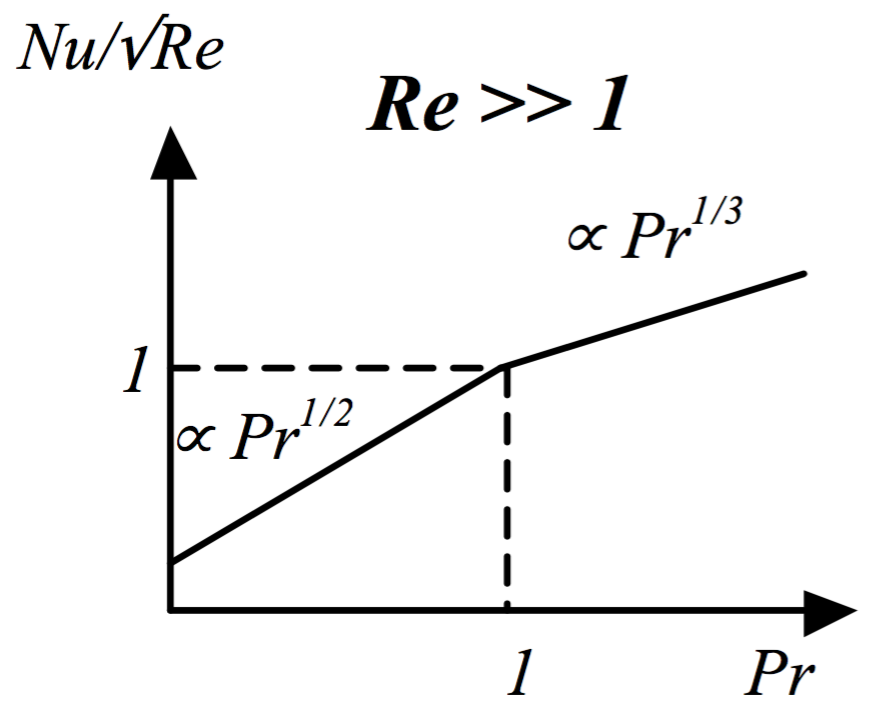
\includegraphics[scale=0.3]{ch5/9}
			\end{flushright}
		\end{minipage}
		\begin{minipage}{0.5\textwidth}
		%	\begin{flushright}
				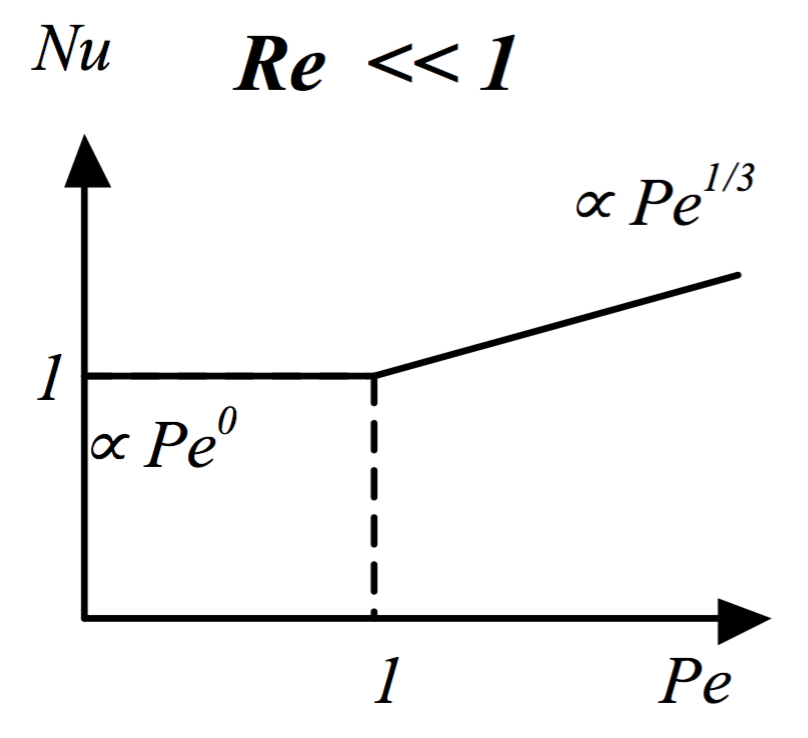
\includegraphics[scale=0.3]{ch5/10}
			%\end{flushright}
		\end{minipage}
		
\section{The Colburn-Chilton analogy}
	In forced convection, it is important to know the friction coefficient $f$ (shear stress) and $Nu$ number (heat transfer rates). It's so usefull to have a relation linking the two. These relations are known as \textbf{Colburn-Chilton} analogy. 
	
	\subsection{Relation between f and Nu}
	Let's begin with the expression of the friction coefficient. We will approximate the shear stress like $|\tau _{xy}|_{y=0} \approx \mu\frac{U}{\delta}$ giving
	\begin{equation}
		f = \frac{|\tau _{xy}|_{y=0}}{\frac{1}{2}\rho U^2} = \frac{\mu |\frac{\D u}{\D y}|_{y=0}}{\frac{1}{2}\rho U^2} \approx \frac{\mu \frac{U}{\delta}}{\frac{1}{2}\rho U^2} \qquad \Rightarrow \qquad \delta = \frac{2\nu}{fU}
	\end{equation}
	We will make appear the $Re$ number ($Re = \frac{UR}{\nu}$) by dividing the previous equation by the radius
	\begin{equation}
		\frac{\delta}{R} = \frac{2}{fRe}
	\end{equation}
	We wll now express the Nusselt number (see subsection \ref{subsec:5.3.1}) differently, using the radius as distance $L$
	\begin{equation}
		Nu = \frac{hR}{k} = \frac{R}{\delta _T} = \frac{R}{\delta}\frac{\delta}{\delta _T} \qquad \Rightarrow \qquad Nu = \frac{fRe}{2}\frac{\delta}{\delta _T}
	\end{equation}
	Colburn concluded his analysis saying that $\delta _T = \delta$ but we've seen it's not the case. Chilton added the dimensional analysis for $Pr \gg 1$ ($Pr > 0.5$ in application) and $Pr \ll 1$
	\begin{equation}
		Pr \gg 1 : \frac{\delta }{\delta _T} = Pr ^{\frac{1}{2}} \qquad and \qquad Pr \ll 1 : \frac{\delta}{\delta _T} = Pr ^{\frac{1}{3}}
	\end{equation}

\subsection{Applications}
	See slides 35 and 36 for lecture. All the mathematical expression are on the formula sheet. 
	
\section{Natural convection}
	\subsection{Definition}
		\begin{wrapfigure}[11]{l}{2.5cm}
		\vspace{-5 mm}
		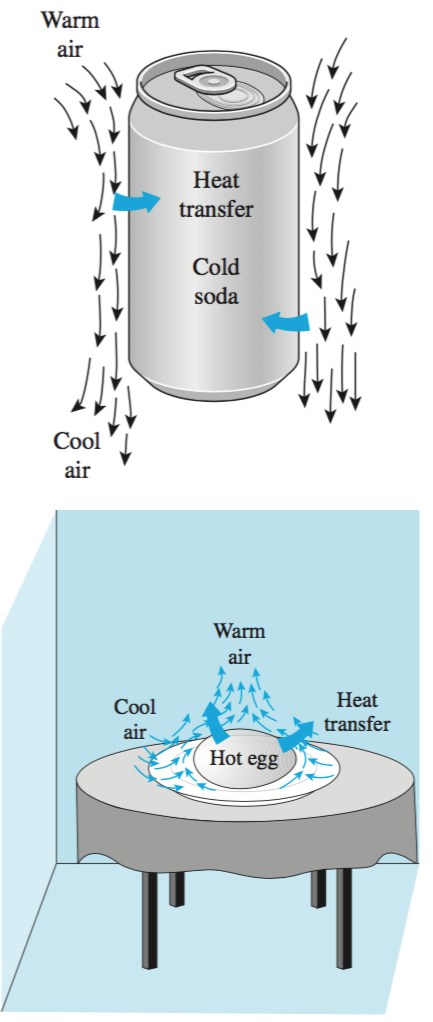
\includegraphics[scale=0.3]{ch5/11}
		\end{wrapfigure}			
		It's probably something that we experience ourself everyday. In forced convection we have to put an external force (ex : impose a pump). This type of convection is not caused by a pomp in a pipe, there is no velocity gradient. Here it is function of the density gradient (a temperature difference or a non-homogeneous concentration field are origins of density changes).\\ 
Imagine that you have a coca can. The warmer air coming to the can will be cooled and directed below (due to air density change). This will create a natural convection process. It’s the opposite for the egg. \\
This is the most complex process you can find. We can’t describe the one without the other (natural and forced).\\

	\subsection{The Navier-Stokes equations}
		We can adapt the Navier-Stokes equations to the case of a natural convection. For a fluid at temperature $T$, concentration $c$ and $\rho$ a function of $(T,c)$
		\begin{equation}
			\rho \frac{D v}{D t} = -\nabla p + \rho g + \nabla \tau
		\end{equation}
		we define the dynamic pressure P, in respect with a reference state. $\rho _0$ is a reference density calculated at a reference temperature and concentraiton
		\begin{equation}
			\nabla P = \nabla p - \rho _0 g \qquad with \qquad \rho _ 0 = \rho (T_0,c_0)
		\end{equation}
		The resulting equation
		\begin{equation}
			\rho \frac{D v}{D t} = -\nabla P + (\rho - \rho _0) g + \nabla \tau
		\end{equation}		 
		stresses\footnote{Insister sur} the role of the term reponsible for the natural convection (density gradient). 

		\subsubsection{The Boussinesq hypothesis}
			We will first assume that the density gradient is smaller than the reference density, leading to $\frac{\Delta \rho }{\rho _0} \ll 1$. 
			We will secondly assume that the density varies linearly with temperature and solute concentration 
			\begin{equation}
				\rho = \rho _0 - \rho \beta _T (T-T_0) - \rho \beta _c (c-c_0)
			\end{equation}
			where $\beta _T$ is the \textbf{temperature expansion coefficient} and $\beta _c$ the \textbf{concentration expansion coefficient} given by 
			\begin{equation}
				\beta _T = - \frac{1}{\rho} \left( \frac{\D \rho}{\D t} \right) _{p,c} \qquad and \qquad \beta _c = - \frac{1}{\rho} \left( \frac{\D \rho}{\D c} \right) _{p,T}
			\end{equation}
			The minus sign here is necessary because the density decreses with temperature and solute concentration. 
			
		\subsubsection{Pure fluid}
			For a \textbf{pure ideal gas} there is no notion of concentration so 
			\begin{equation}
				\beta _T = \frac{RT}{pM} \frac{pM}{RT^2} = \frac{1}{T} \qquad and \qquad \beta _c = 0
			\end{equation}
			The density changes so only in function of the temperature 
			\begin{equation}
				\frac{\rho _0}{\rho} = 1 + \beta _T (T-T_0)
			\end{equation}
			Knowing that the continuity equation gives us the informatino $\nabla v = 0$, the Navier-Stokes equations become
			\begin{equation}
				\frac{Dv}{Dt} = \frac{\D v}{\D t} + v\nabla v = - \frac{1}{\rho _0} \nabla P - (T-T_0) \beta _T g + \nu \nabla ^2 v
				\label{eq:5.62}
			\end{equation}
			In addition to that, we have the energy conservation equation
			\begin{equation}
				\frac{DT}{Dt} = \frac{\D T}{\D t} + v \nabla T = \alpha \nabla ^2 T 
			\end{equation}
	\subsection{Channel flow}
		\begin{wrapfigure}[9]{l}{2.5cm}
		\vspace{-5 mm}
		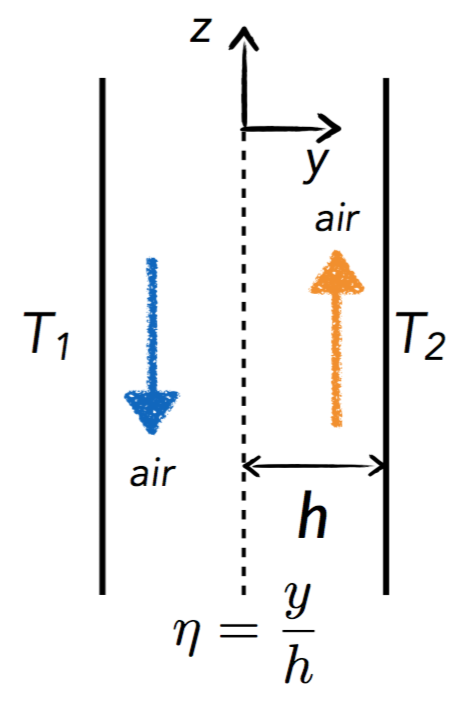
\includegraphics[scale=0.3]{ch5/12}
		\end{wrapfigure}			
		This is one of the few problems with an exact solution. Let's consider a channel of length $L=2h$, infinite height, $v_z = v(y)$ and $T_z = T(y)$. There are 2 walls, one cold $T_1$ and the other hot $T_2 = T_1 + \Delta T$. The fluid in contact with the colder one will move down and the other up. Finally, there is also conduction in $y$ direction respecting a linear $T$ profile. \\
		Let's now begin with the Fourrier law and let's apply the boundary conditions
		\begin{equation}
			\frac{\D ^2 T}{\D t^2} = 0  \qquad and \qquad 
			\left\{ 
			\begin{aligned}
				y =- h \qquad T &= T_1 \\
				y = h \qquad T &= T_2
			\end{aligned}
			\right.
		\end{equation}
		The result is 
		\begin{equation}
			\tilde{T} (\eta ) = \frac{T-T_m}{\Delta T} = \frac{1}{2} \eta \qquad where \qquad T_m = \frac{T_1 + T_2}{2}
		\end{equation}
		
	\subsubsection{The Navier-Stokes equations in z direction}
		Let see what happens to Navier-Stokes equations. Here is the full version 
		\begin{equation}
			\cancel{\left( u\frac{\D v}{\D y} + v\frac{\D v}{\D z} \right)} = - \frac{1}{\rho} \frac{\D P}{\D z} - (T-T_0)\beta _T g + \nu \left( \cancel{\frac{\D ^2 v}{\D z^2}} + \frac{\D ^2 v}{\D y^2} \right)
		\end{equation}
		We don’t have variation of $v$ in the directions $y$ and $z$. We only have one diffusion term in $y$ direction. Let's introduce the non dimentional velocity and length
		\begin{equation}
			\tilde{v} = \frac{v}{\frac{\nu}{h}} \qquad and \qquad \eta = \frac{y}{h}
		\end{equation}
	 	Let's now do the modification to make appear these expressions
	 	\begin{equation}
	 		\frac{\nu ^2}{h^3} \frac{d^2 \tilde{v}}{d \eta ^2} = \frac{1}{\rho (T_m)} \frac{dP}{dz} - \frac{1}{2} \eta \Delta T \beta _T g \qquad \Leftrightarrow \qquad 
	 		\frac{d^2 \tilde{v}}{d \eta ^2} = \frac{h^3}{\nu ^2\rho (T_m)} \frac{dP}{dz} - \frac{\eta}{2} \underbrace{\frac{h^3 \Delta T \beta _T g}{\nu ^2}}_{Gr}
	 	\end{equation}
		where $Gr$ is the \textbf{Grashof number}. Using the non-		sleep condition at the wall ($\tilde{v} = 0$), we have the 	profile 
		\begin{equation}
			\tilde{v} (\tilde{\eta}) = \frac{1}{12} Gr (\eta - \eta ^3) - \frac{h^3}{2\nu ^2\rho (T_m)} \frac{dP}{dz} (1-\eta ^2)
		\end{equation}
		valid only in the case of a \textbf{constant pressure gradient}. The first term is the \textbf{Buoyancy term}, a cubic velocity profile with zero mean velocity and the second is the \textbf{Pressure term}, the quadratic Poiseuille velocity profile. Extreamly complex ! 
		
		\subsubsection{The mean velocity}
			\begin{wrapfigure}[5]{l}{3.2cm}
			\vspace{-5 mm}
			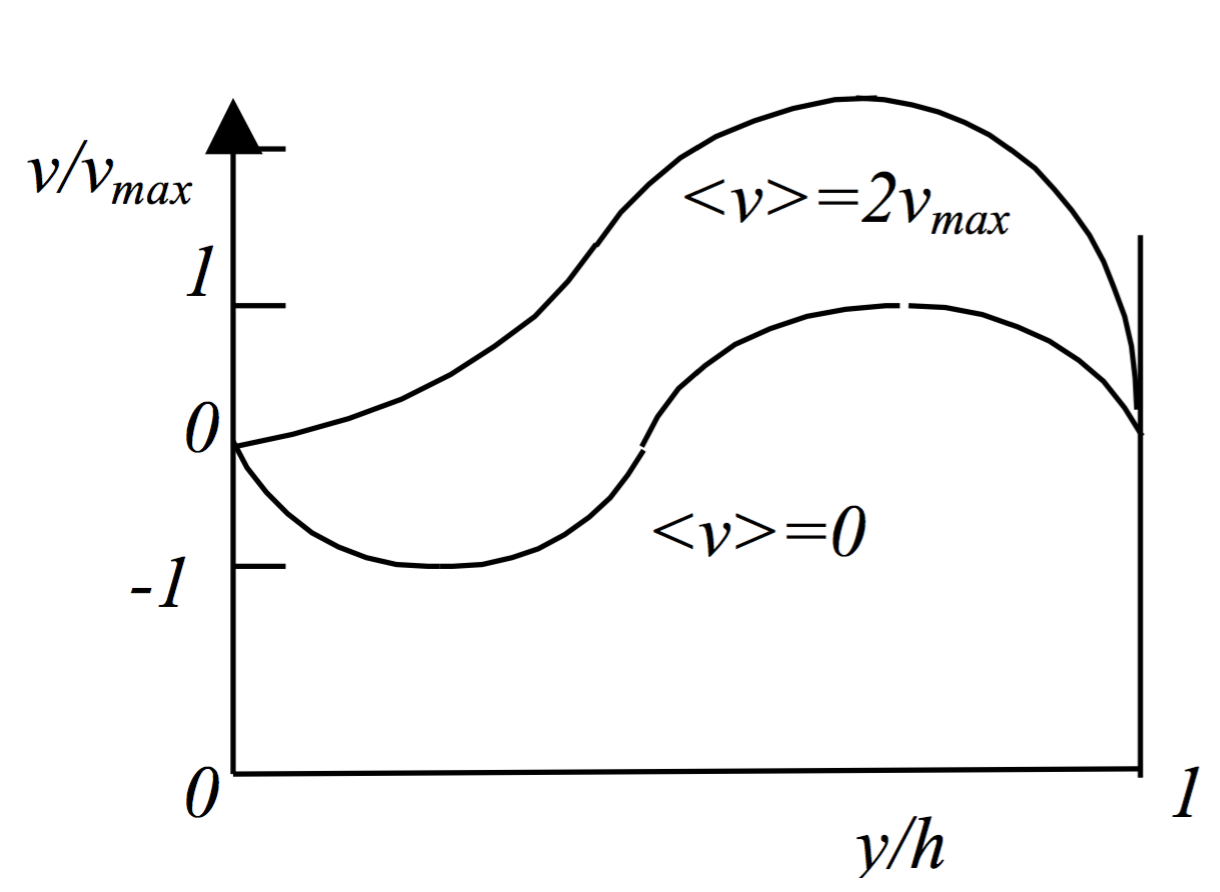
\includegraphics[scale=0.15]{ch5/13}
			\end{wrapfigure}		
		We don't know the pressure gradient so we introduce the mean velocity to determine it
			\begin{equation}
				<\tilde{v}> = \frac{1}{2} \int _{-1} ^1 \tilde{v} (\eta) \, d\eta = - \frac{h^3}{3\nu ^2\rho (T_m)} \frac{dP}{dz} 
			\end{equation}
			If $<\tilde{v}> = 0$ the pressure definition contains an average buoyancy term, so $P = c$. If $<\tilde{v}> \neq 0$, it's the general case where the net flux in the $z$ direction exists. The velocity profile is represented on the left.
		
\subsection{Dimentional analysis}
	Let's see a little bit in terms of scalings how we behave in natural convection. A classic situation is the case of a body of temperature $T_0 = T_\infty + \Delta T$ and air around it with temperature $T_\infty$. The buoyancy term can be equilibrated by viscous forces or inertial forces, depending on the Reynolds number. We remind the Navier-Stokes equations \ref{eq:5.62} and consider \\
	\begin{itemize}
		\item[•] $Re \ll 1$ : Buoyancy term equilibrated by viscous forces (channel flow problem)
		\begin{equation}
			\nu \frac{U_{cv}}{L^2} = g \beta _T \Delta T \qquad \Rightarrow \qquad U_{cv} = \frac{L^2 g \beta _T \Delta T}{\nu}
		\end{equation}
		
		\item[•] $Re \gg 1$ : Buoyancy term equilibrated by inertial forces
		\begin{equation}
			\frac{U^2_{c}}{L} = g\beta _T \Delta T \qquad \Rightarrow \qquad U_c = \sqrt{L g \beta _T \Delta T}
		\end{equation}
	\end{itemize}
	
	\subsubsection{Non-dimentional forms of the Navier-Stokes equations for Re << 1}
	The non-dimentional terms are
	\begin{equation}
		U_{cv} = \frac{L^2 g \beta _T \Delta T}{\nu} \qquad \tilde{v} = \frac{v}{U_{cv}} \qquad \tilde{T} = \frac{T-T_\infty}{\Delta T} \qquad \tilde{P} = \frac{P}{\frac{\mu U_{cv}}{L}} \qquad \tilde{r} = \frac{r}{L}
	\end{equation}
	Transforming the Navier-Stokes equations in (non-dimentional)
	\begin{equation}
		Gr \, \tilde{v} \cdot \tilde{\nabla} \tilde{v} = - \tilde{\nabla} \tilde{P} - \tilde{T} 1_g + \tilde{\nabla ^2} \tilde{v} \qquad where \qquad \tilde{\nabla} = L\nabla \qquad and \qquad 1_g = \left( 
		\begin{array}{c}
		0 \\ 
		0 \\ 
		-1
		\end{array} 
		\right)
	\end{equation}
	The $Gr = \frac{L^3 \beta _T g \Delta T}{\nu ^2}$. If $Gr \ll 1$ the inertial term can be omitted but it happens seldom. $Re \ll 1$ is equivalent to $Gr \ll 1$. 
	
	\subsubsection{Non-dimentional forms of the Navier-Stokes equations for Re >> 1}
	The non-dimentional terms are
	\begin{equation}
		U_{c} = \sqrt{L g \beta _T \Delta T} \qquad \tilde{v} = \frac{v}{U_{cv}} \qquad \tilde{T} = \frac{T-T_\infty}{\Delta T} \qquad \tilde{P} = \frac{P}{\rho U^2_c} \qquad \tilde{r} = \frac{r}{L}
	\end{equation}
	Transforming the Navier-Stokes equations in (non-dimentional)
	\begin{equation}
		\tilde{v} \tilde{\nabla} \tilde{v} = - \tilde{\nabla} \tilde{P} - \tilde{T} 1_g + \frac{1}{Gr ^{\frac{1}{2}}} \tilde{\nabla ^2} \tilde{v} \qquad where \qquad \tilde{\nabla} \tilde{v}= 0 \qquad and \qquad \tilde{v} \tilde{\nabla} \tilde{T} = \frac{1}{Pr Gr^{\frac{1}{2}}} \tilde{\nabla}^2 \tilde{T}
		\label{eq:5.76}
	\end{equation}
	In this case, $Gr = \frac{L^3\beta _T g \Delta T}{\nu ^2} = \left( \frac{U_c L}{\nu}\right) ^2= Re^2 $. If $Gr \gg 1$ the viscous term can be omitted and the condition $Re \gg 1$ is equivalent to $Gr \gg 1$.
	
	\section{The natural convection thermal boundary layer}
		In natural convection, Re is replaced by Gr, so a momentum boundary layer will form when $Gr \gg 1$. At the edge of the boundary layer, convection and conduction are of the same order of magnitude. Using \autoref{eq:5.76}, we can approximate
		\begin{equation}
			\frac{1}{Gr^{\frac{1}{2}}}\tilde{\nabla}^2 \tilde{v} \approx \frac{1}{Gr^{\frac{1}{2}}} \frac{1}{\tilde{\delta}^2} \approx \frac{1}{Gr^{\frac{1}{2}}} \frac{L^2}{\tilde{\delta}^2} \approx 1 \qquad \Rightarrow \qquad \frac{\delta}{L} \approx \frac{1}{Gr^{\frac{1}{4}}} 
		\end{equation}
		Result equivalent to the Blasius solution for momentum
    	The velocity profile in natural convection is not approximately linear as in forced convection, due to the presence of a buoyancy term. \\
    	
		A thermal boundary layer of thickness $\delta _T$ is established when $Pr Gr^{0.5} \gg 1$ (equivalent to $Pe \gg 1$) 
		\begin{equation}
			\tilde{v} \tilde{\nabla} \tilde{T} = \frac{1}{Pr Gr^{\frac{1}{2}}} \tilde{\nabla}^2 \tilde{T}
		\end{equation}
		\begin{itemize}
		\item[•]	If $Pr \ll 1$, $\delta _T \gg \delta$, the fluid is outside the momentum boundary layer. Using
		\begin{equation}
			\tilde{v}\approx 1 \qquad \tilde{v}\tilde{\nabla}\tilde{T} \approx 1
		\end{equation}
		We approximate
		\begin{equation}
			\frac{1}{Pr Gr^{\frac{1}{2}}} \frac{1}{\tilde{\delta} _T^2}\approx 1 \qquad \Rightarrow \qquad \tilde{\delta _T} = \frac{\delta _T}{L} = Gr^{-\frac{1}{4}}Pr^{-\frac{1}{2}}
		\end{equation}
		Result equivalent to the solution for forced convection. 
		
		\item[•] If $Pr \gg 1$, $\delta _T \ll \delta$, the fluid is inside the momentum boundary layer (velocity profile not known). For a given $Gr$, $\delta _T$ will decrease with $Pr$ and $v$ will decrease at the thermal boundary layer border 
		\begin{equation}
			\frac{\delta _T}{\delta} = Pr ^{-a} \qquad \tilde{v} = Pr ^{-b}
		\end{equation}
		
		At the border of thermal boundary layer, the viscous term equilibrates the driving force
		\begin{equation}
		\frac{1}{Gr ^{\frac{1}{2}}} \tilde{\nabla} ^2 \tilde{v} \approx 1 \Rightarrow \frac{1}{Gr ^{\frac{1}{2}}} \frac{\tilde{v}}{\tilde{\delta}_T ^2} \approx Pr ^{2a-b} \approx 1 \qquad \Rightarrow \qquad 2a - b = 0 
		\end{equation}
		In addition to that 
		\begin{equation}
			\tilde{v} \tilde{\nabla} \tilde{T} \approx \tilde{v} \approx Pr ^{-b} =\frac{1}{PrGr ^{\frac{1}{2}}}\tilde{\nabla}^2 \tilde{T} = \frac{1}{PrGr ^{\frac{1}{2}}} \frac{1}{\tilde{\delta}_T^2} \approx Pr^{-1+2a} \qquad \Rightarrow \qquad 2a +b = 1
		\end{equation}
		The combination of the two equations gives the values of $a = 0.25$ and $b = 0.5$.
		\end{itemize}
		
	\subsubsection{Relation between the momentum and thermal boundary layer thickness}
	For $Gr \gg 1$
	\begin{equation}
		\frac{\delta _T}{L} \approx \frac{\delta }{L}Pr ^{-\frac{1}{4}} = Gr ^{-\frac{1}{4}}Pr ^{-\frac{1}{4}} = Ra ^{-\frac{1}{4}}
	\end{equation}
	where $Ra$ is the \textbf{Rayleigh number} 
	\begin{equation}
		Ra = GrPr = \frac{L^3 g \beta _T \Delta T}{\nu ^2}\frac{ \nu }{\alpha} = \frac{L^3 g \beta _T \Delta T}{\nu \alpha}
	\end{equation}
	Finally, the Nusselt number is given by
	\begin{equation}
		Nu = \frac{L}{\delta _T} =C \cdot Gr ^{\frac{1}{4}}Pr ^{\frac{1}{4}} = Ra ^{\frac{1}{4}}
	\end{equation}